%!TEX root = ../thesis.tex
%*******************************************************************************
%*********************************** Background estimation *********
%*******************************************************************************


\chapter{Background estimation}

\ifpdf
    \graphicspath{{chapter-background/Figs/Raster/}{chapter-background/Figs/PDF/}{chapter-background/Figs/}}
\else
    \graphicspath{{chapter-background/Figs/Vector/}{chapter-background/Figs/}}
\fi

\glsreset{cr}

A reliable estimation of the expected \gls{sm} background rates in the \glspl{sr} is crucial for exercising the statistical machinery laid out in \cref{ch:statistics} and making conclusive statistical statements. The background estimation approaches used in the following either rely on semi-data-driven techniques or on \gls{mc}-only estimations. As estimating backgrounds only from \gls{mc} simulation is often problematic due to \eg mis-modelings in the phase space regions targeted not appropriately covered by the uncertainties, a (semi-)data-driven approach is often favoured. In the following, the major backgrounds $\ttbar$, single top and $\wjets$ are estimated using a semi-data-driven approach, while the expected rates from the remaining smaller backgrounds rely purely on \gls{mc} simulations and are normalised to their theoretical cross section.

\section{General strategy}

\subsection{Transfer factor approach}

Estimating background contributions in \glspl{sr} in a semi-data-driven approach, usually involves the introduction of so-called \glspl{cr} used to control dominant background processes by comparing their expected event rates to data. The \glspl{cr} are designed to be enriched in events of a given background process (or type) while being approximately free of signal contamination. If $N_p^\mathrm{MC}(\mathrm{SR})$ and $N_p^\mathrm{MC}(\mathrm{CR})$ are the expected rates for a given background process $p$ from \gls{mc} simulation in a given \gls{sr} and \gls{cr}, respectively, then the transfer factor $N_p^\mathrm{MC}(\mathrm{SR})/N_p^\mathrm{MC}(\mathrm{CR})$ allows to convert the number of observed background events in the \glspl{cr}, $N_p^\mathrm{obs.}(\mathrm{CR})$ into a background estimate in the \glspl{sr},$N_p^\mathrm{est.}(\mathrm{SR})$, through
\begin{equation}
	N_p^\mathrm{est.}(\mathrm{SR}) = N_p^\mathrm{obs.}(\mathrm{CR}) \frac{N_p^\mathrm{MC}(\mathrm{SR})}{N_p^\mathrm{MC}(\mathrm{CR})} = \mu_p N_p^\mathrm{MC}(\mathrm{SR}).
	\label{eq:transfer_factor}
\end{equation}
An important benefit of this approach is that the impact of systematic uncertainties on the estimated background rates can be evaluated on the transfer factors, that are ratios of \gls{mc} estimates. As such, systematic uncertainties can be canceled in the extrapolation to the \gls{sr}. The uncertainty on the background estimate is then a combination of statistical uncertainties in the \gls{cr} and remaining uncertainties affecting the extrapolation. For this reason, \glspl{cr} are usually deliberately chosen to have large statistics, effectively reducing the uncertainties on the extrapolation to the \glspl{sr}.  

As indicated in~\cref{eq:transfer_factor}, the transfer factor approach is formally equivalent to using the process-specific normalisation factor introduced in~\cref{sec:likelihood_function}, effectively \textit{normalising} the number of background events expected from \gls{mc} in the \gls{cr} to the number of observed events. In the profile likelihood fit setups used in the following, implemented using \textsc{HistFitter}~\cite{HistFitter:2014wma}, the normalisation factor $\mu_b$ is fitted to data instead of background as expected from \gls{mc} simulation. In the following, multiple disjoint \glspl{cr} are used to simultaneously normalise multiple background processes to data in a combined fit. In order not to have an underdetermined minimisation problem, at least the same number of \glspl{cr} as normalisation factors needs to be used. Two different profile likelihood fit configurations are used in the following, a \textit{background-only} fit configuration assuming no signal contribution and typically only including the \glspl{cr}, and a \textit{model-dependent} fit configuration with nominal signal contribution using \glspl{cr} as well as \gls{sr}.

In order to verify the quality of the extrapolation from the \glspl{cr} to the \glspl{sr}, so-called \gls{vr} are defined. \glspl{vr} do not participate in the actual fit of the model parameters to data, but serve as intermediate regions to verify the extrapolation. For this reason, \glspl{vr} are typically placed in the region between the \glspl{cr} and \glspl{sr} that is extrapolated over. A schematic view of an analysis strategy using all three types of regions is shown in~\cref{fig:hf_strategy}. All three types of regions can have more than one bin and are separated using suitable observables that are extrapolated over.


\begin{figure}
\floatbox[{\capbeside\thisfloatsetup{capbesideposition={right,center},capbesidewidth=0.5\textwidth}}]{figure}[\FBwidth]
{\caption{Schematic view of an analysis strategy including multiple control, validation and signal regions with one or multiple bins each. Extrapolations from the control regions into the signal regions can be verified in the validation regions lying in the phase space extrapolated over. Figure adapted from~\cite{HistFitter:2014wma}.}\label{fig:hf_strategy}}
{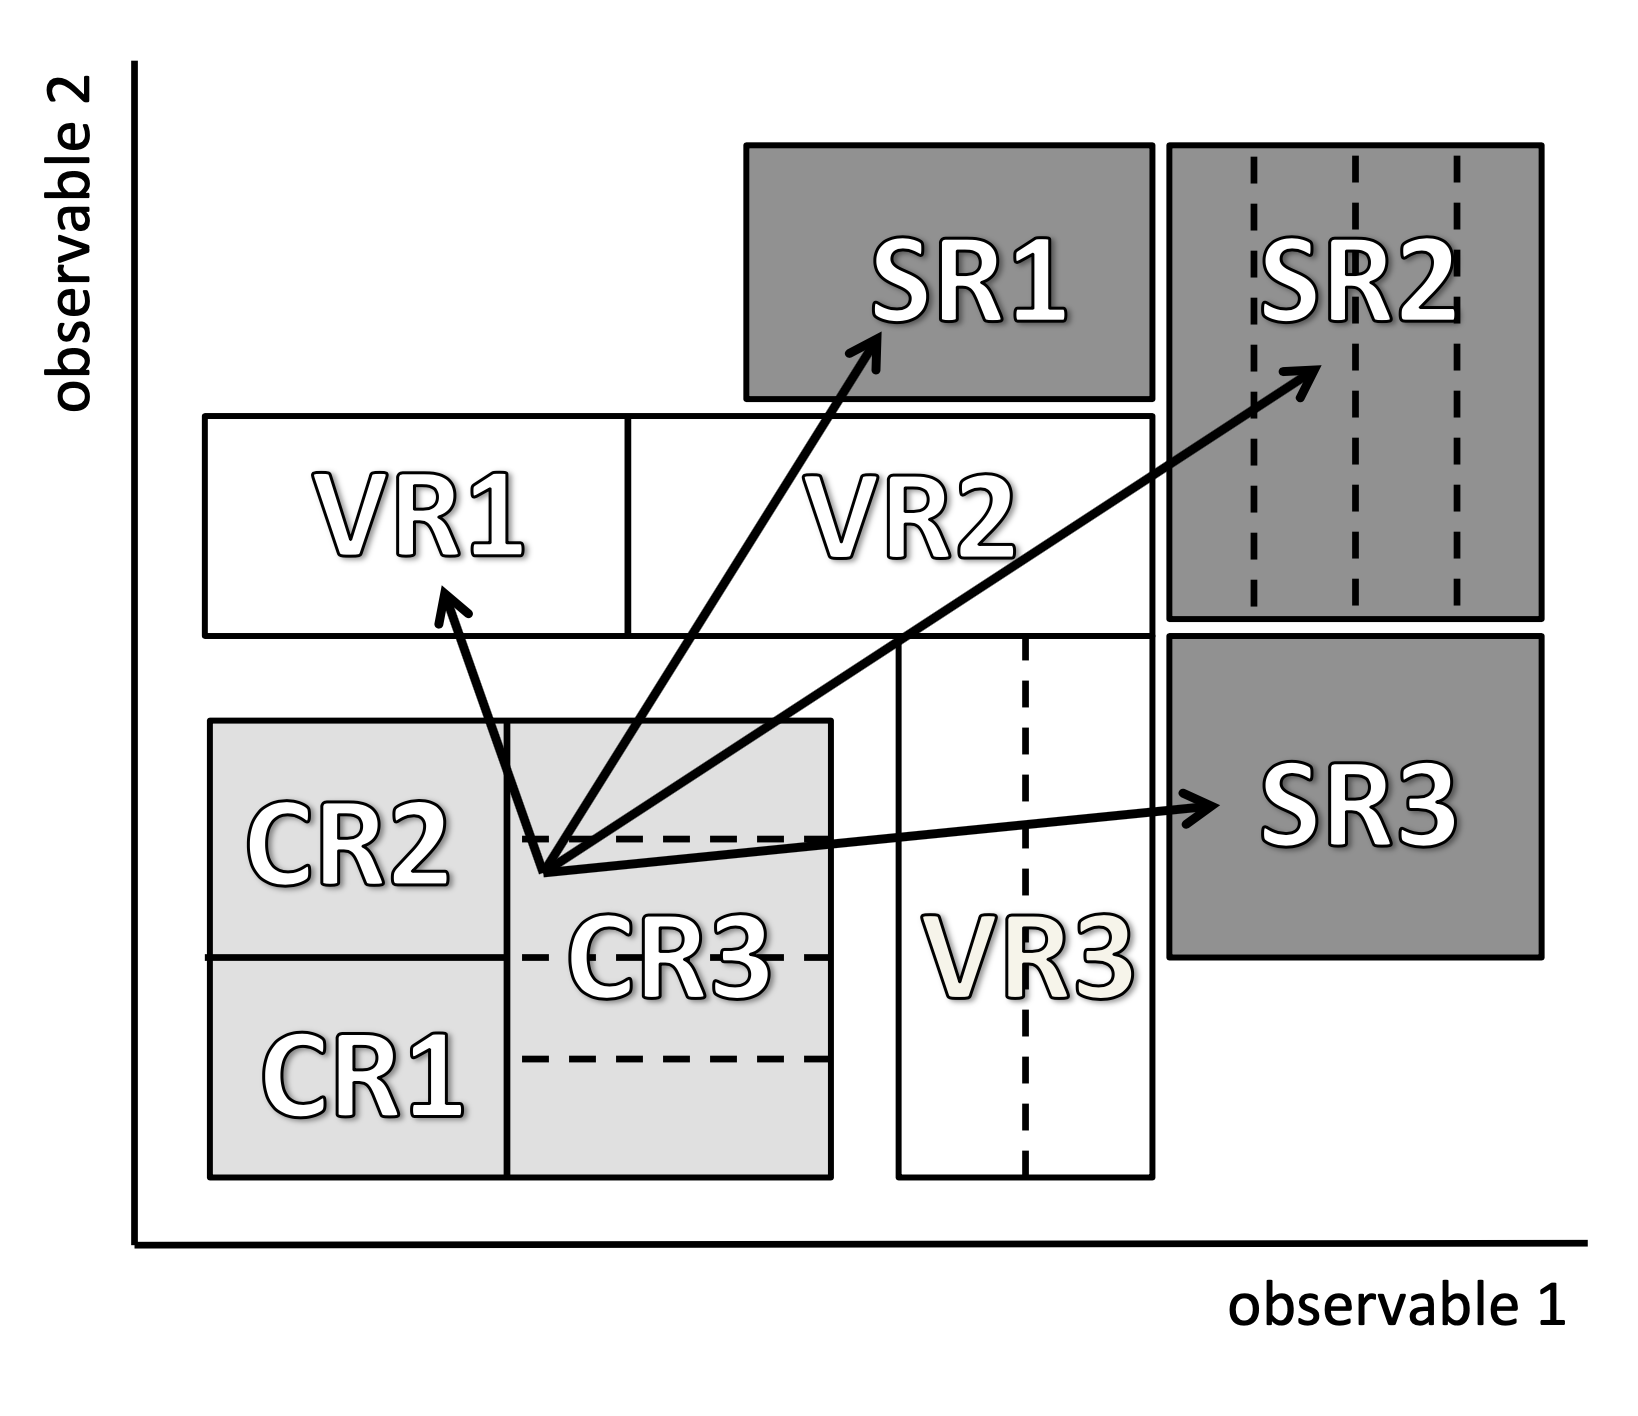
\includegraphics[width=0.45\textwidth]{hf_strategy}}
\end{figure}

\subsection{Analysis blinding}

An important concept in the design phase of searches for new physics is the idea of \textit{blinding} regions of interest~\cite{blind:2003rw}, meaning that measured data are not looked at in these regions. This avoids issues of \textit{experimenter's bias}, \ie unintended influences on the design of the analysis based on the observed data. If data were already known when designing the signal regions (and therefore the outcome of the analysis would be known to some extent), experimenter's bias could for example occur during the selection of the final signal region definitions.

During the design of a search for new physics, signal regions are generally kept blinded until the complete analysis strategy is fixed. Once the \glspl{sr} have been designed, the next step is to develop suitable \glspl{cr} with negligible signal contamination. This is followed by design of \glspl{vr} that can be unblinded once the \glspl{cr} are fixed. The \glspl{sr} are only unblinded after the extrapolation from the \glspl{cr} has been verified in the \glspl{vr}, allowing to either quantify potential excesses in data or set limits on model parameters. 

\subsection{Data versus Monte Carlo plots}

In this chapter, all plots comparing data versus \gls{mc} are \textit{pre-fit}, meaning that no background-only fit has been run in order to determine the normalisation factors and total systematic uncertainties for the background estimate. The contributions from the dominant backgrounds $\ttbar$, $\wjets$ and single top are normalised simultaneously in the control regions by solving the system of $i$ equations
\begin{equation}
%	\begin{split}
		n_\mathrm{data}^{\mathrm{CR}_i} = \mu_{\ttbar} B_{\ttbar}^{\mathrm{CR}_i} + \mu_{W} B_{W}^{\mathrm{CR}_i} + \mu_\mathrm{ST} B_\mathrm{ST}^{\mathrm{CR}_i} + B_\mathrm{other}^{\mathrm{CR}_i},
%	\end{split}
\end{equation}
where $i$ runs over the list of \glspl{cr} introduced in \cref{sec:control_regions} and $\mu_{\ttbar}$, $\mu_\mathrm{W}$ and $\mu_\mathrm{ST}$ are the normalisation factors of the $\ttbar$, $\wjets$ and single top backgrounds, respectively, that are to be determined. $B_{\ttbar}^{\mathrm{CR}_i}$, $B_\mathrm{ST}^{\mathrm{CR}_i}$, $B_\mathrm{ST}^{\mathrm{CR}_i}$ and $B_\mathrm{other}^{\mathrm{CR}_i}$ are the background rates expected from \gls{mc} simulation in the \textit{i}-th \gls{cr}. Normalisation factors obtained are 0.96 for $\ttbar$, 1.24 for $\wjets$ and 0.73 for single top. As will be shown in~\cref{sec:results_background_only}, the normalisation factors obtained using the full statistical procedure will be close to these values.

Additionally, the uncertainty bands on the background estimation include only \gls{mc} statistical uncertainty as well as experimental uncertainties. The variations of the experimental uncertainties are normalised to the nominal background estimate in the case of $\ttbar$, $\wjets$ and single top, such that only the shapes of the dominant backgrounds are affected. For the remaining minor backgrounds, the experimental uncertainties can affect both normalisation and shape. All experimental uncertainties are assumed to be fully correlated over all processes and bins, allowing them to be added together in quadrature. The uncertainty bars on the data points correspond to the 68\% confidence interval, assuming data to be Poisson distributed. 

\section{Control regions}\label{sec:control_regions}

\begin{table}
\begin{center}
\resizebox{\textwidth}{!}{
\begin{tabular} {l | c c c | cccccc}
\toprule
\textbf{CR} & \textbf{TR-LM} &  \textbf{TR-MM} &  \textbf{TR-HM} &  \multicolumn{3}{c}{\textbf{WR}} & \multicolumn{3}{c}{ \textbf{STR}} \\                 
\midrule
$\mbb$ [$\GeV$]  & \multicolumn{3}{c|}{$<$100 or $>$140} & \multicolumn{3}{c}{$\in[50,80]$} &\multicolumn{3}{c}{$>$195}\\
$\mt$ [$\GeV$]   & $\in[100,160]$ & $\in[160,240]$ & $>$240 & \multicolumn{3}{c}{$\in[50,100]$} &\multicolumn{3}{c}{$>$100}\\
$\mct$ [$\GeV$]  &\multicolumn{3}{c|}{$<$180} & \multicolumn{3}{c}{$>$180} &\multicolumn{3}{c}{$>$180}\\
\midrule
\textbf{VR} & \textbf{VR-onLM} &  \textbf{VR-onMM} & \textbf{VR-onHM} & \multicolumn{2}{c}{ \textbf{VR-offLM}} &  \multicolumn{2}{c}{\textbf{VR-offMM}} &  \multicolumn{2}{c}{\textbf{VR-offHM}}\\
\midrule
$\mbb$ [$\GeV$]  & \multicolumn{3}{c|}{$\in[100,140]$} & \multicolumn{2}{c}{$\in[50,80]\, \cup [160, 195]$} & \multicolumn{2}{c}{$\in[50,80]\, \cup [160, 195]$}& \multicolumn{2}{c}{$\in[50,75]\, \cup [165, 195]$}\\
$\mt$ [$\GeV$]   & $\in[100,160]$ & $\in[160,240]$ & $>$240 & \multicolumn{2}{c}{$\in[100,160]$} & \multicolumn{2}{c}{$\in[160,240]$} & \multicolumn{2}{c}{$>$240}\\
$\mct$ [$\GeV$]  &\multicolumn{3}{c|}{$<$180}&\multicolumn{6}{c}{$>$180}\\
\bottomrule
\end{tabular}}
\caption{Overview of the CR and VR definitions. All regions partially share the same selection as the SR for all variables except $\mlb$, which is not used in the CR and VR definitions.} 
\label{tab:CRVRdef}
\end{center}
\end{table}

The contributions from $\ttbar$, $\wjets$ production and single top processes are normalised to data in dedicated \glspl{cr}. Other processes like $Z+\mathrm{jets}$, diboson and multiboson, $\ttbar+V$, $\ttbar+h$ and $V+h$ are estimated directly from \gls{mc} simulation and normalised to their theoretical cross sections. All \glspl{cr} are designed to be kinematically as close as possible to the respective \glspl{sr}, such that the normalisation factors derived in the \glspl{cr} are also valid in the \glspl{sr}. The \glspl{cr} are mutually exclusive and made orthogonal to the \glspl{sr} through their requirements on $\mt$, $\mct$ and $\mbb$. Apart from the requirements on these three observables as well as the requirement on $\mlb$ (removed altogether in the \glspl{cr}), the \glspl{cr} share the same set of cuts as the \glspl{sr}. \Cref{fig:cr_strategy} illustrates the configuration of all \glspl{cr}, especially highlighting the fact that all \glspl{cr} are located in sideband regions off the $\mbb$ window, significantly reducing signal contamination. \Cref{tab:CRVRdef} summarises the kinematic requirements separating the \glspl{cr} from other regions of interest in the analysis. 

\subsubsection[Control regions for $\ttbar$]{Control regions for $\boldsymbol{\ttbar}$}

As events from $\ttbar$ processes constitute the dominant \gls{sm} background in all \glspl{sr}, it is necessary to have a precise and reliable estimation of their contributions. Three \glspl{cr} are defined for $\ttbar$, following the same binning in $\mt$, and thus called TRLM, TRMM and TRHM in the following. A good purity of $\ttbar$ processes as well as the necessary high \gls{mc} are achieved  by inverting the requirements on $\mbb$ and $\mct$. The achieved $\ttbar$ purities are 79.6\% in TRLM, 85.9\% in TRMM and 84.1\% in TRHM. The composition of the different $\ttbar$ decay modes in each \gls{cr} is found to be similar as in the respective \gls{sr}. The maximum signal contamination over the entire signal grid is 0.8\%, 1.1\% and 1.9\% for TRLM, TRMM and TRHM, respectively, and thus negligible. \Cref{fig:signal_contamination_TRLM,fig:signal_contamination_TRMM,fig:signal_contamination_TRHM} show the signal contamination over the entire signal grid. 

\subsubsection[Control region for $\wjets$]{Control region for $\boldsymbol{\wjets}$}

Events from $\wjets$ production represent the second largest contribution of \gls{sm} background events in the \glspl{sr}. A single $\wjets$ \gls{cr} (WR) is defined by replacing the requirements on $\mt$ and $\mbb$ with $\SI{50}{\GeV} < mt < \SI{100}{\GeV}$  and $\SI{50}{\GeV} < \mbb < \SI{80}{\GeV}$, respectively. No bins in $\mct$ are defined for WR. As for the $\ttbar$ control regions, moving WR off the Higgs mass peak allows to achieve a tolerable maximum signal contamination of about 2.4\% (with most signal points having significantly less than 1\% signal contamination in WR), as shown in \cref{fig:signal_contamination_WR}. Applying a low requirement on $\mt$ allows to predominantly select events in front of the kinematic endpoint of the transverse mass of the W boson, resulting in a high statistics control region with a $\wjets$ purity of roughly 52.5\%.

\subsubsection{Control region for single top}

Single top processes result in significant background contributions in some \glspl{sr}, necessitating a proper semi-data-driven estimation. A single top \gls{cr} (STR) is defined by replacing the Higgs mass window cut on $\mbb$ with $\mbb > \SI{195}{\GeV}$ and removing the bins in $\mct$. Off the Higgs mass peak guarantees a low maximum signal contamination of roughly 0.8\% and a high purity of single top processes of about 51.7\%. The signal contamination across the entire signal grid is shown in \cref{fig:signal_contaminations_STCR}.

 \begin{figure}
	\centering
	\begin{subfigure}[b]{0.5\linewidth}
		\centering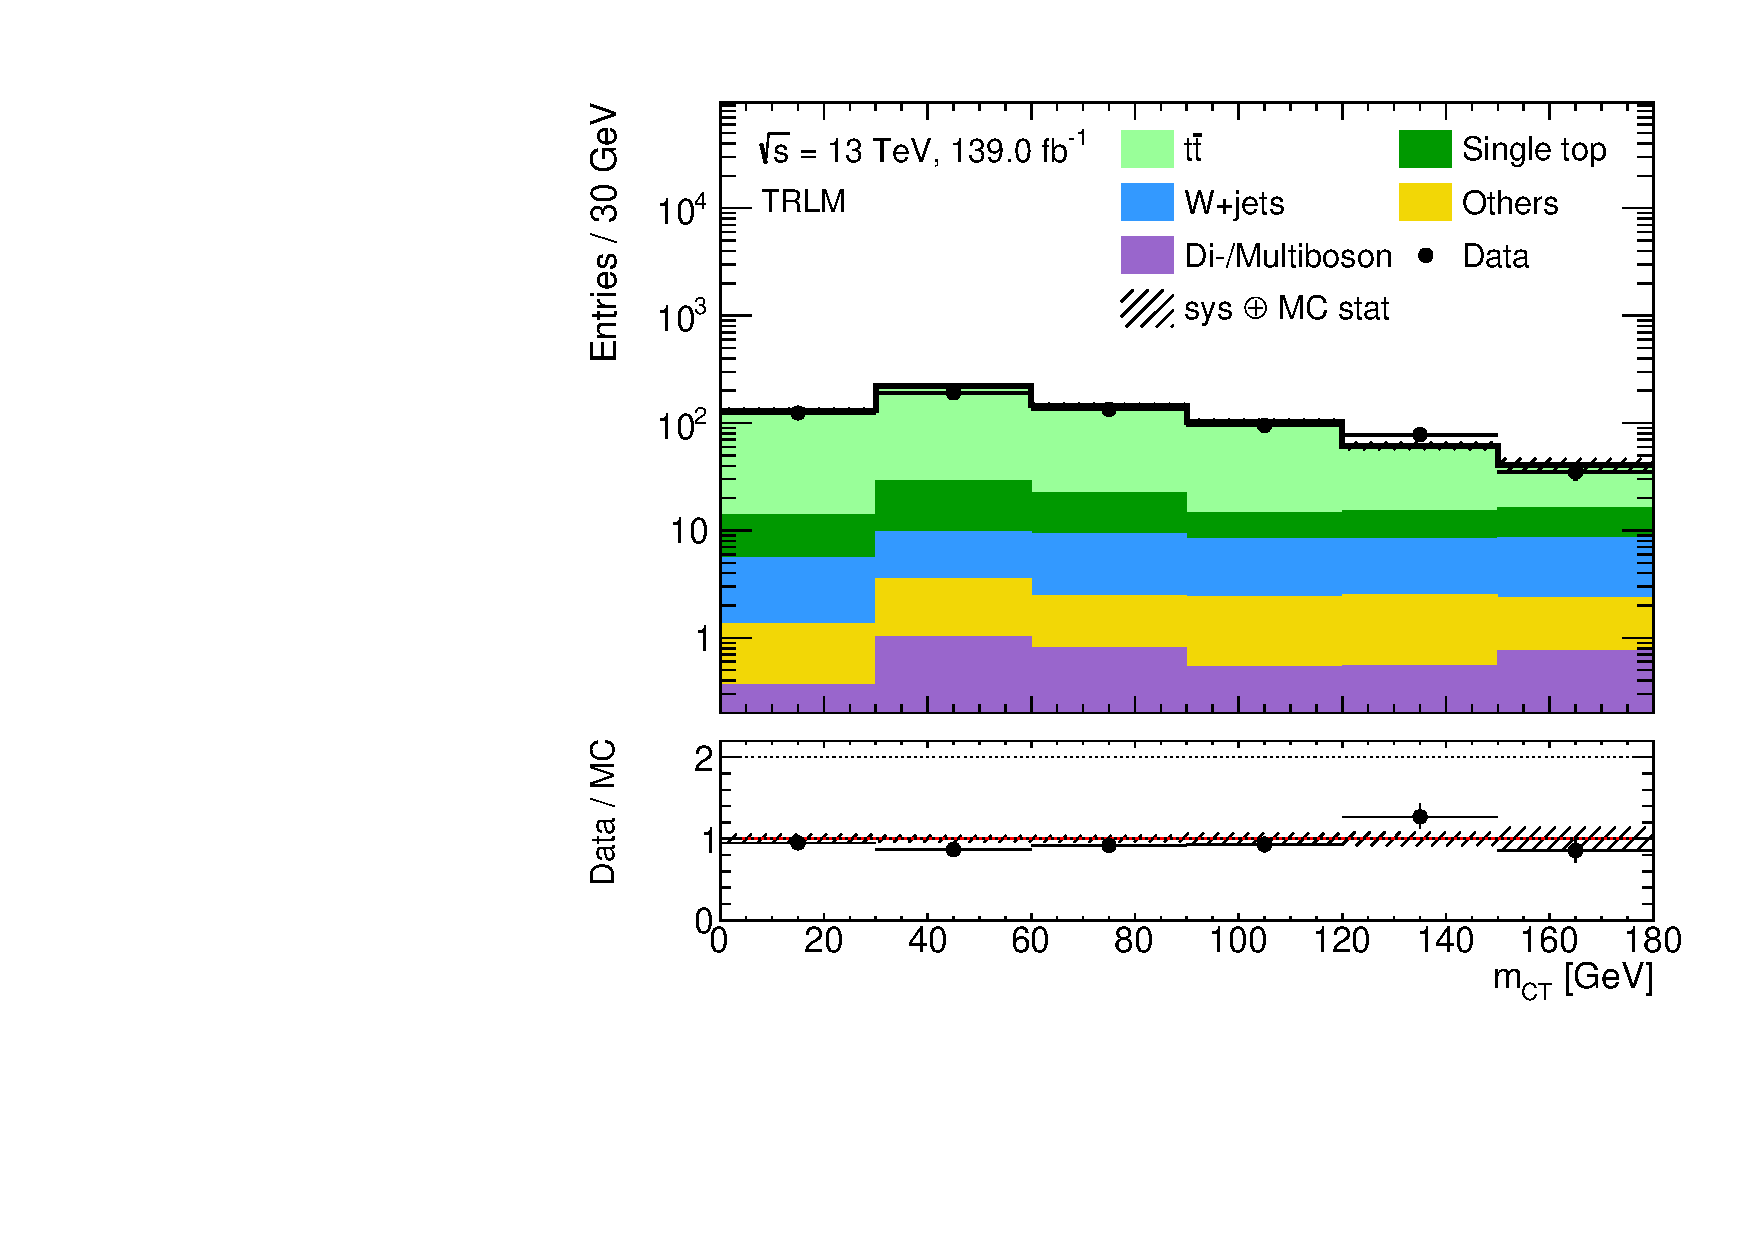
\includegraphics[width=1.0\textwidth]{1Lbb_TRLM_mct}
		\caption{TRLM\label{fig:signal_contamination_TRLM}}
	\end{subfigure}\hfill
	\begin{subfigure}[b]{0.5\linewidth}
		\centering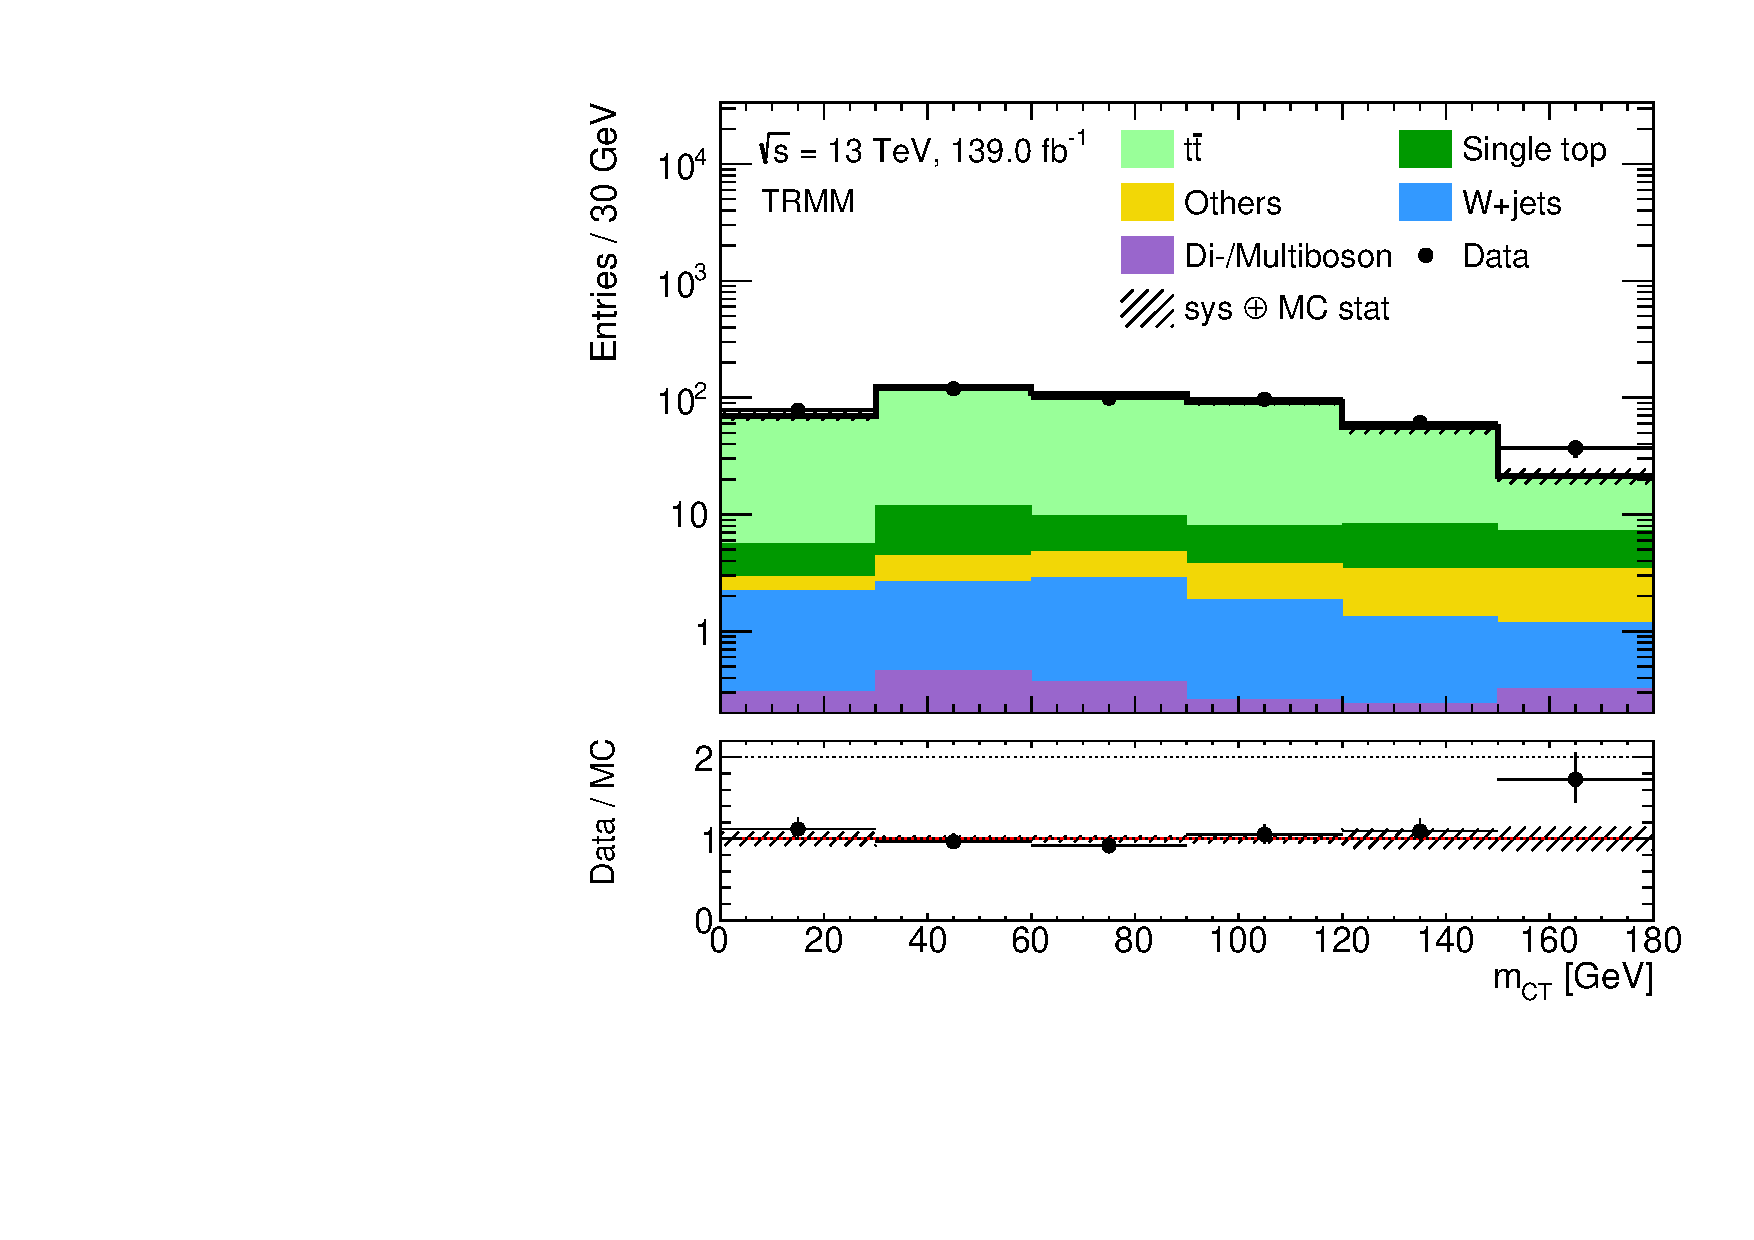
\includegraphics[width=1.0\textwidth]{1Lbb_TRMM_mct}
		\caption{TRMM\label{fig:signal_contamination_TRMM}}
	\end{subfigure}\hfill
	\begin{subfigure}[b]{0.5\linewidth}
		\centering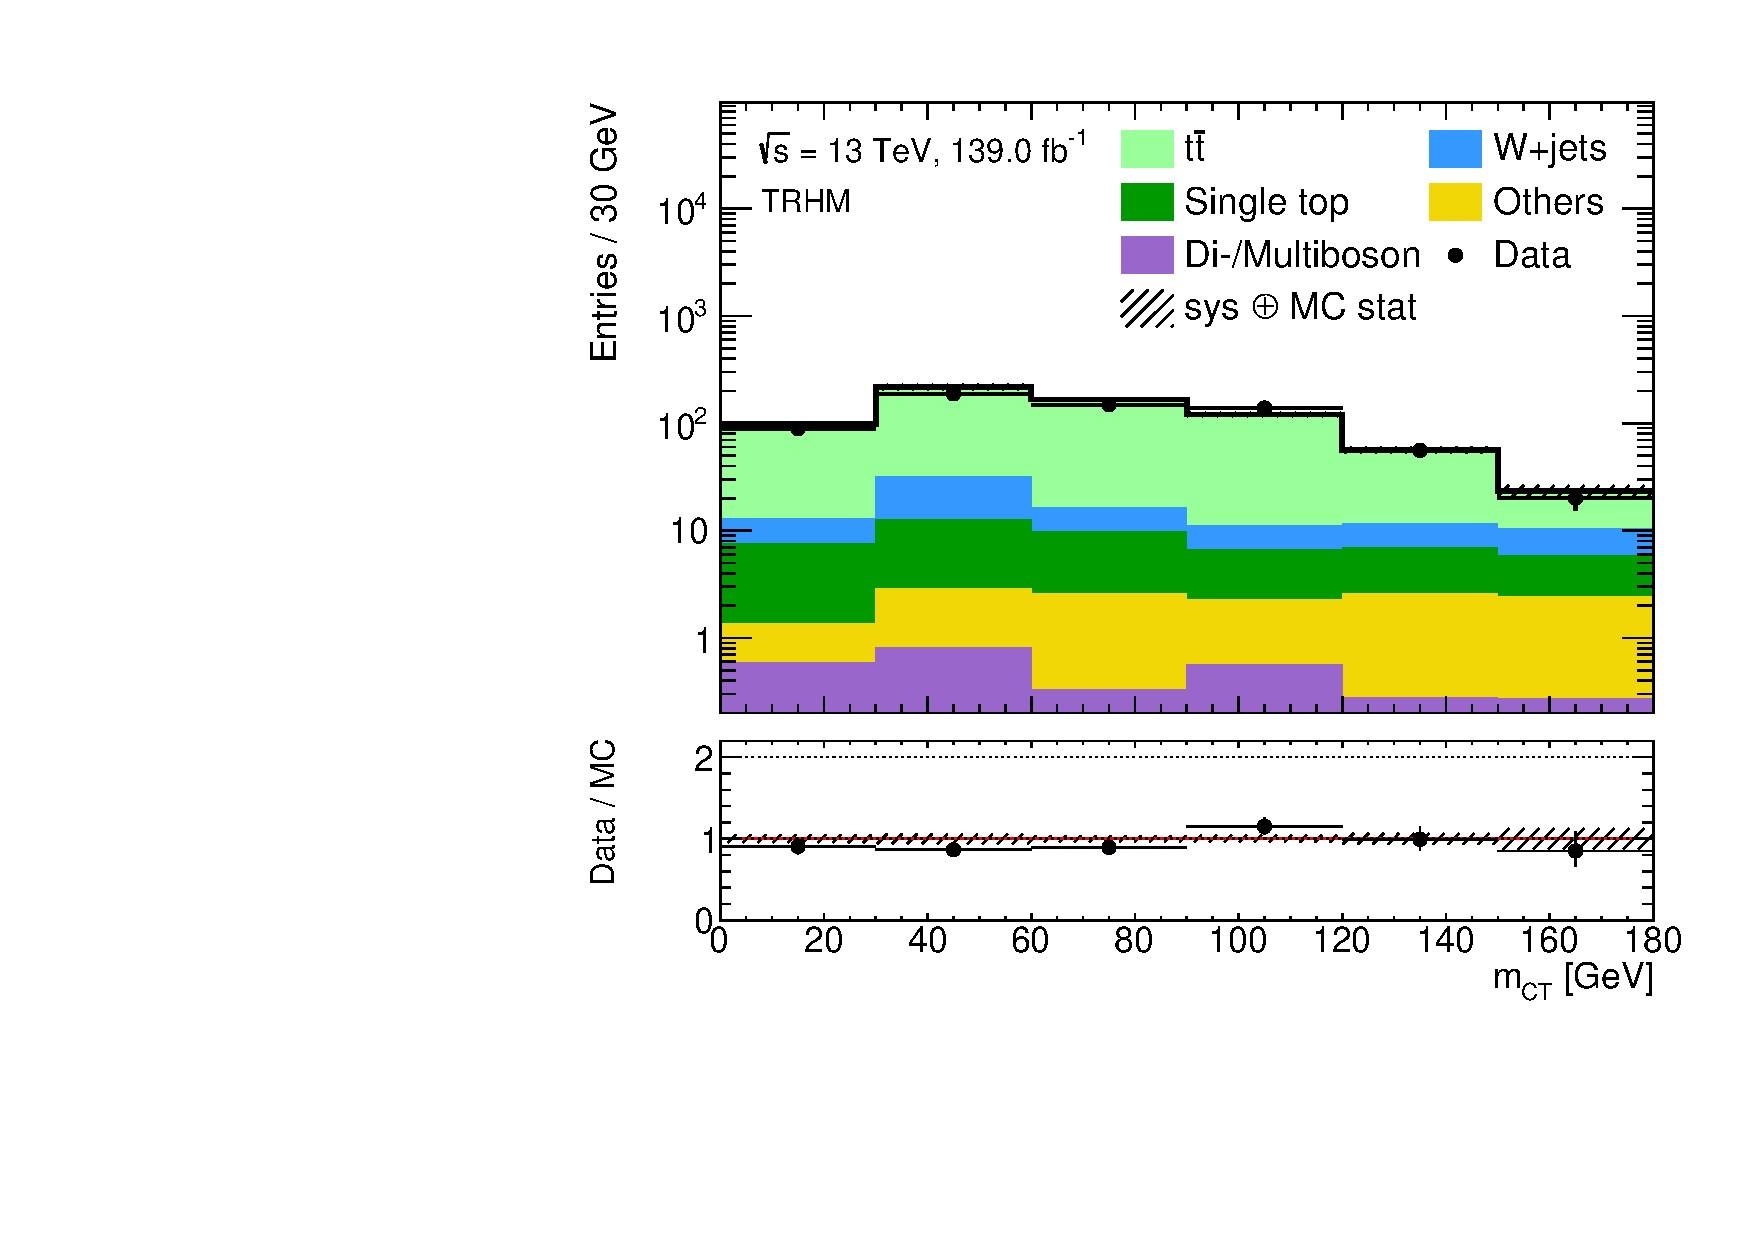
\includegraphics[width=1.0\textwidth]{1Lbb_TRHM_mct}
		\caption{TRHM\label{fig:signal_contamination_TRHM}}
	\end{subfigure}\hfill
	\begin{subfigure}[b]{0.5\linewidth}
		\centering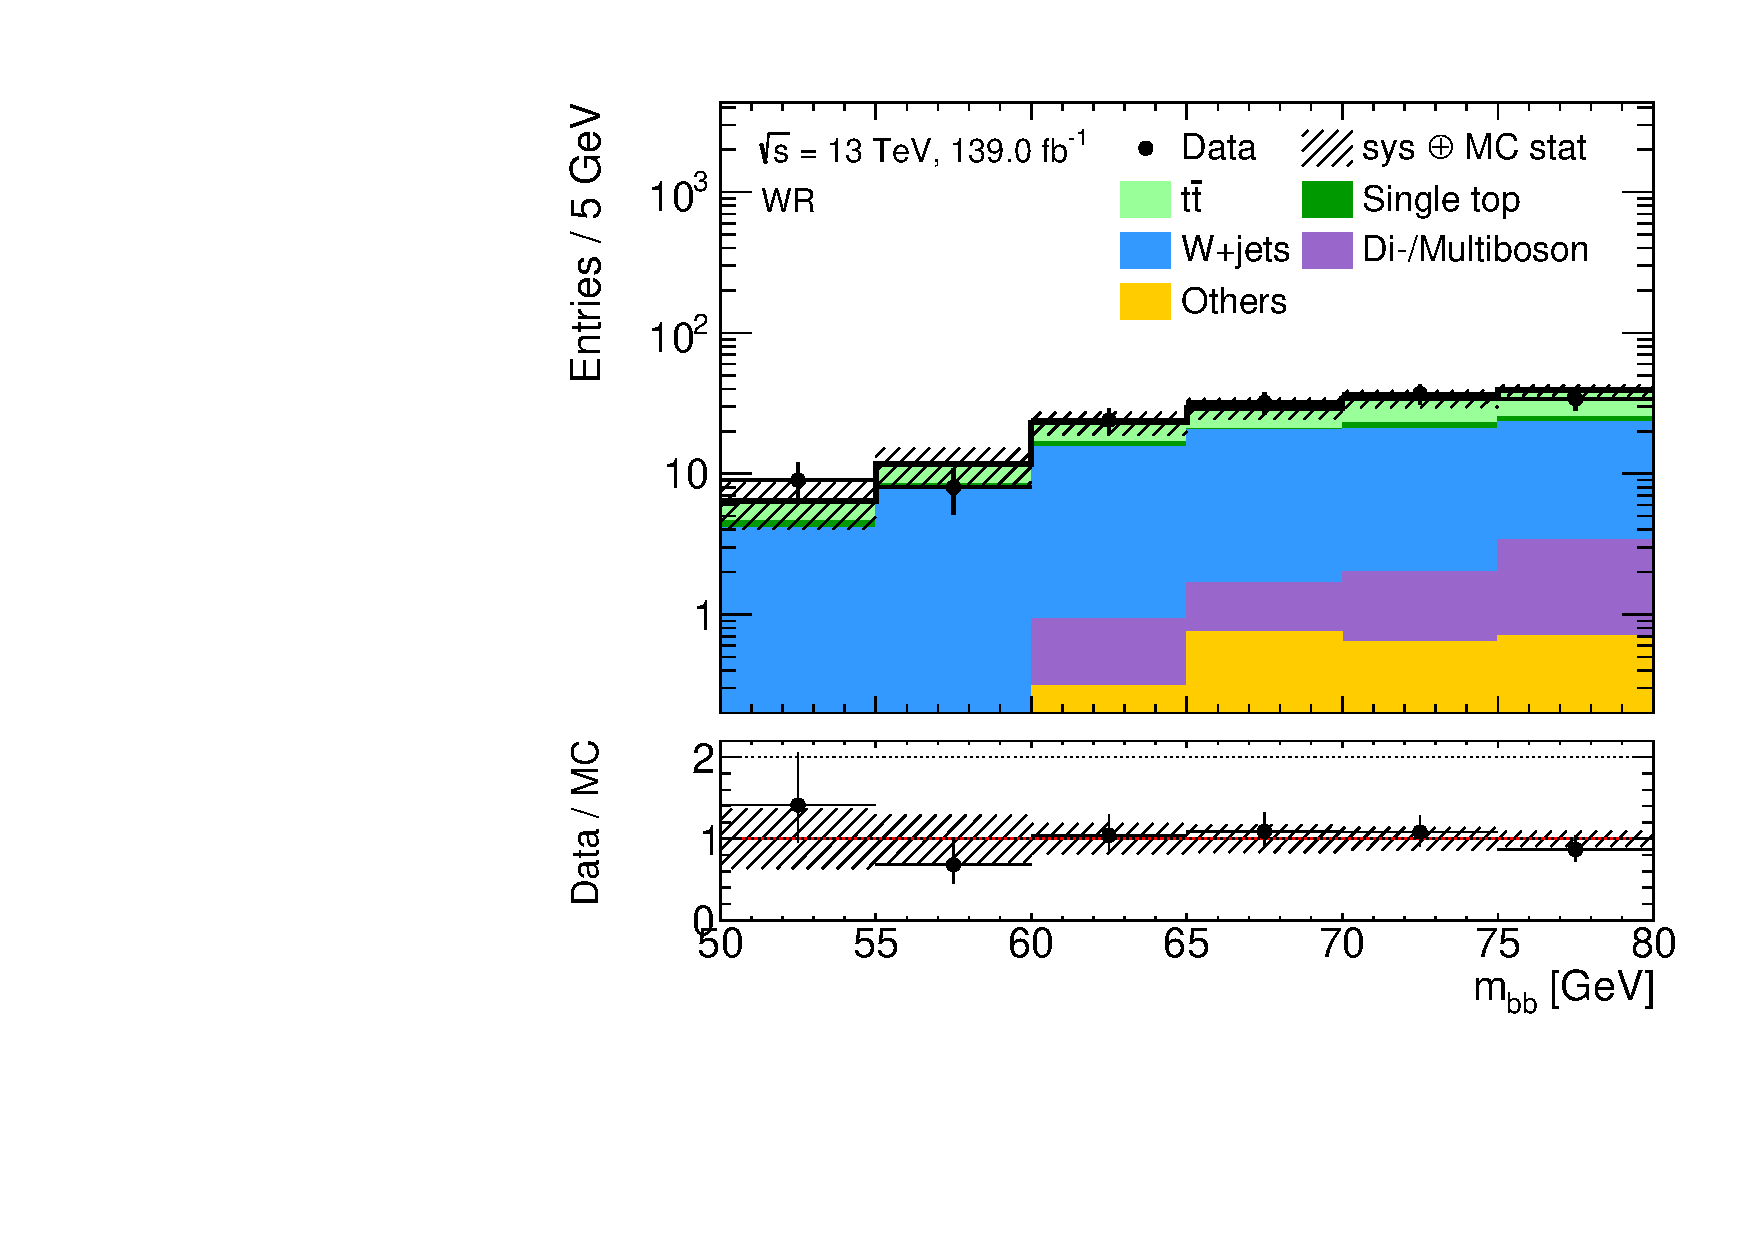
\includegraphics[width=1.0\textwidth]{1Lbb_WR_mbb}
		\caption{WR\label{fig:signal_contamination_WR}}
	\end{subfigure}\hfill
	\begin{subfigure}[b]{0.5\linewidth}
		\centering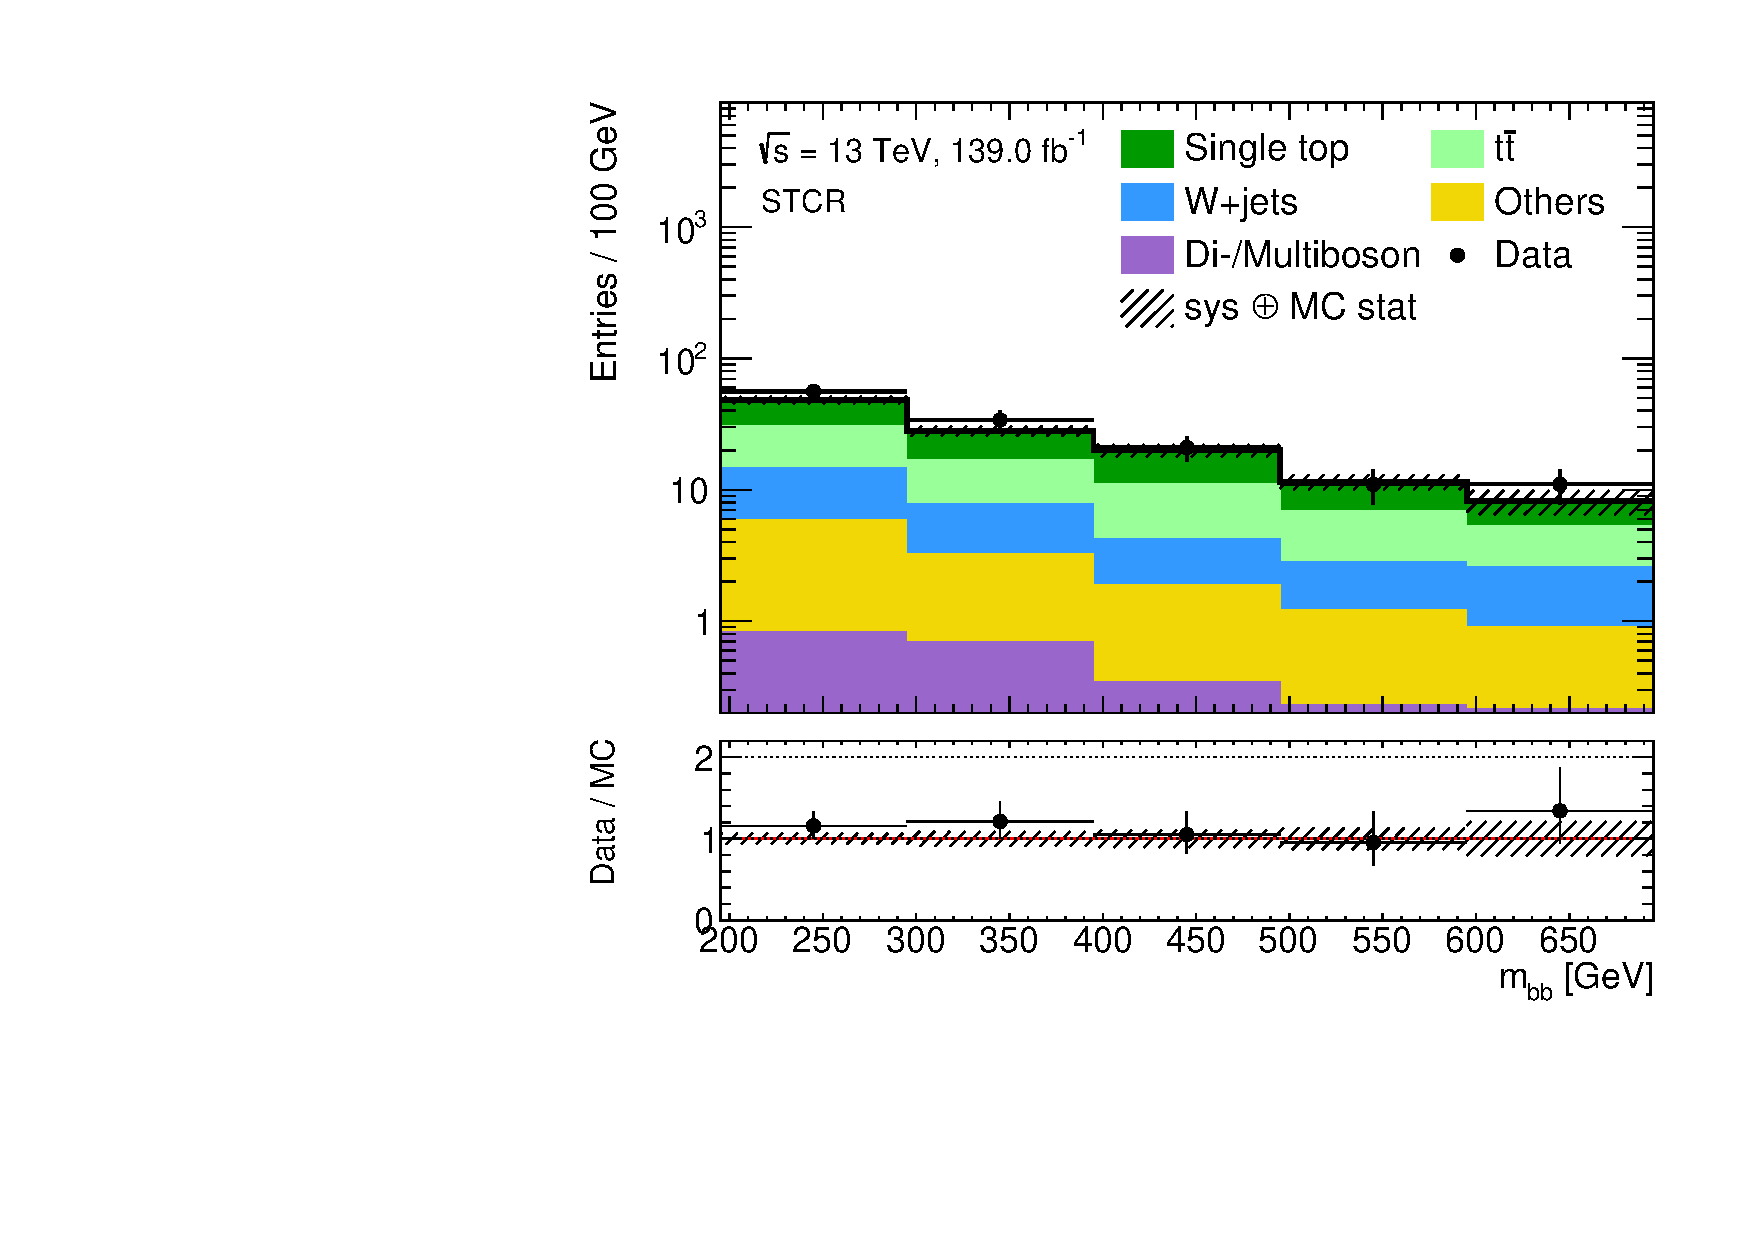
\includegraphics[width=1.0\textwidth]{1Lbb_STCR_mbb}
		\caption{STCR\label{fig:signal_contaminations_STCR}}
	\end{subfigure}\hfill

	\caption{Exemplary distribution shown in each control region. As laid out in the beginning of this chapter, the shaded region includes \gls{mc} statistical uncertainty as well as experimental uncertainties, added in quadrature. A good agreement between \gls{mc} expectation and data is observed in all \glspl{cr}.}
	\label{fig:CR_distributions_prefit}
\end{figure}

 \begin{figure}
	\centering
	\begin{subfigure}[b]{0.5\linewidth}
		\centering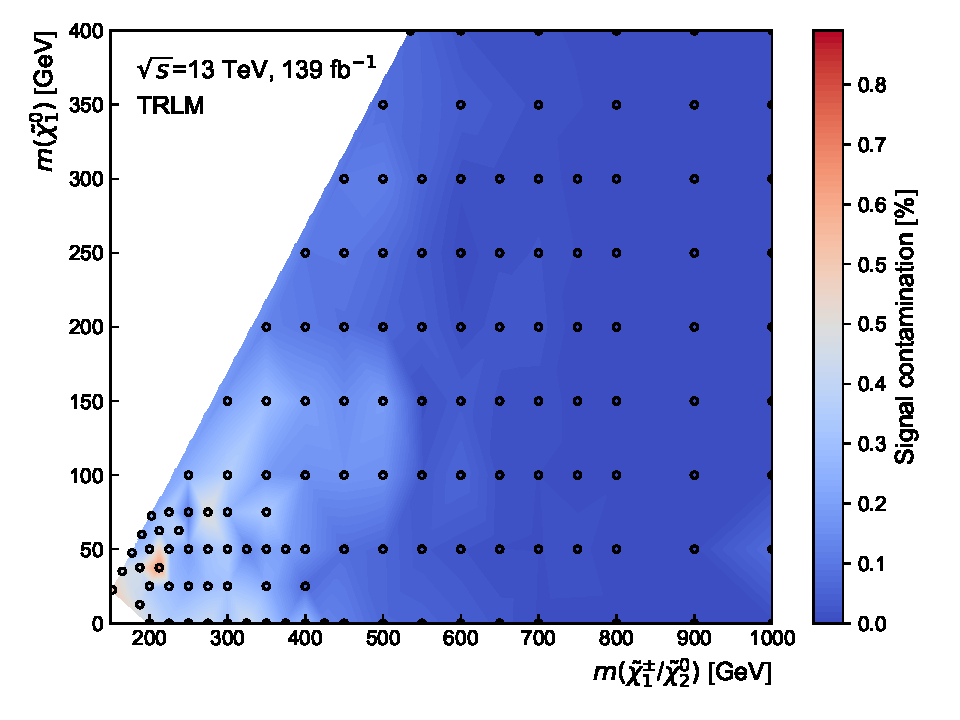
\includegraphics[width=1.0\textwidth]{signal_contamination/plot_TRLM}
		\caption{TRLM\label{fig:signal_contamination_TRLM}}
	\end{subfigure}\hfill
	\begin{subfigure}[b]{0.5\linewidth}
		\centering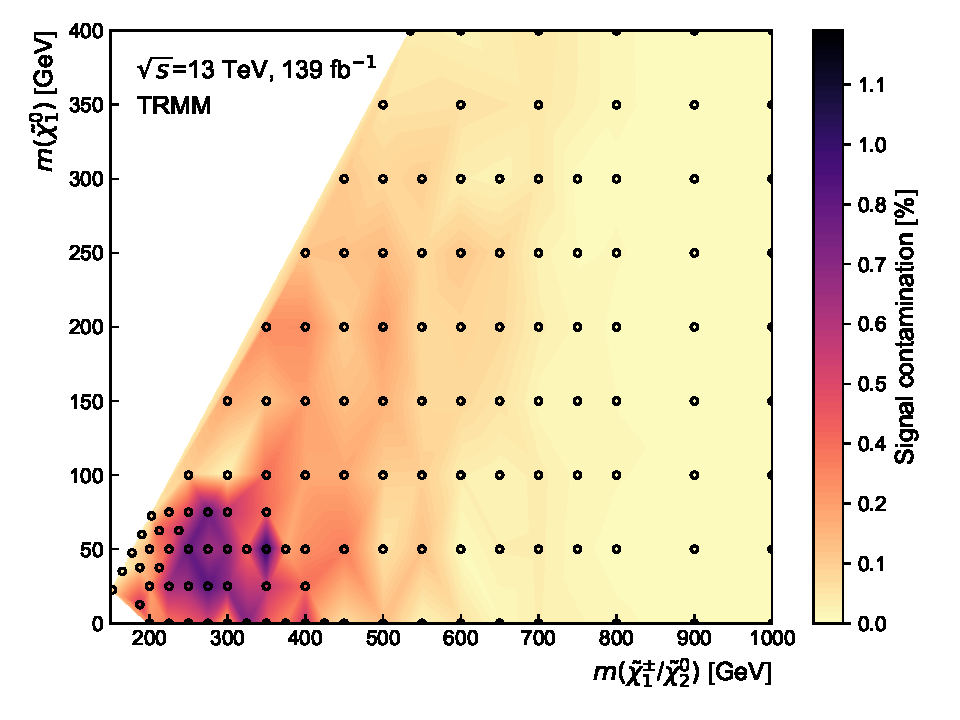
\includegraphics[width=1.0\textwidth]{signal_contamination/plot_TRMM}
		\caption{TRMM\label{fig:signal_contamination_TRMM}}
	\end{subfigure}\hfill
	\begin{subfigure}[b]{0.5\linewidth}
		\centering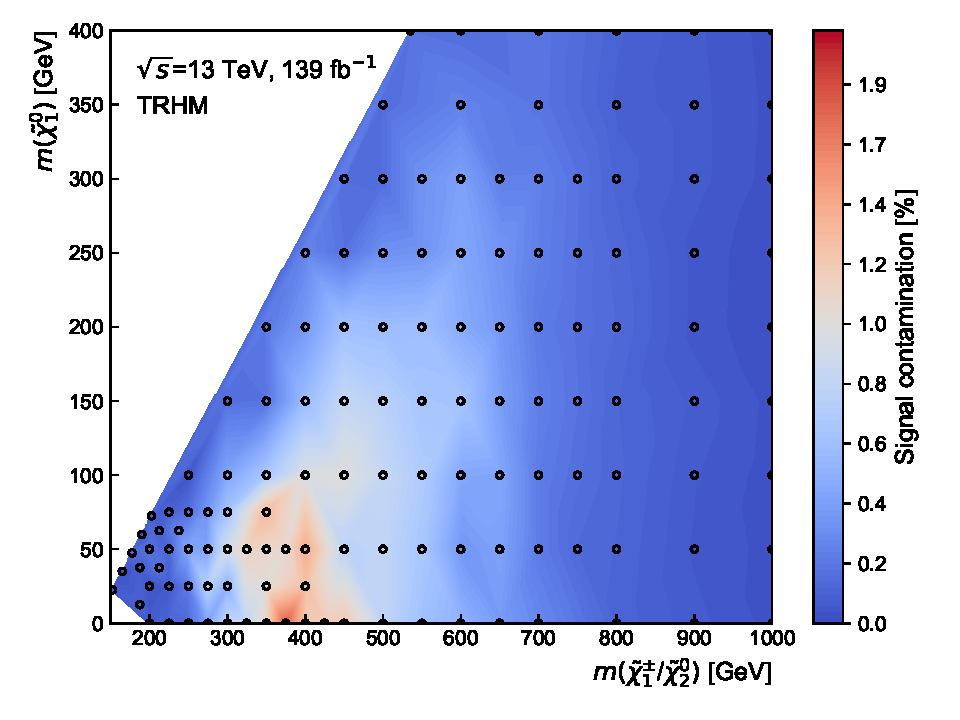
\includegraphics[width=1.0\textwidth]{signal_contamination/plot_TRHM}
		\caption{TRHM\label{fig:signal_contamination_TRHM}}
	\end{subfigure}\hfill
	\begin{subfigure}[b]{0.5\linewidth}
		\centering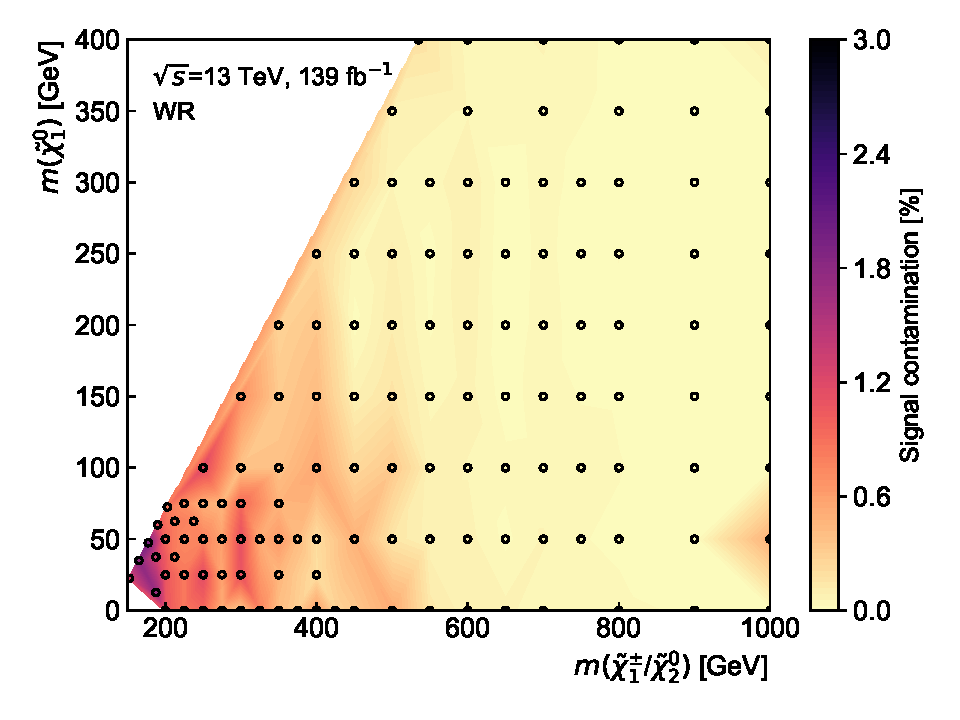
\includegraphics[width=1.0\textwidth]{signal_contamination/plot_WR}
		\caption{WR\label{fig:signal_contamination_WR}}
	\end{subfigure}\hfill
	\begin{subfigure}[b]{0.5\linewidth}
		\centering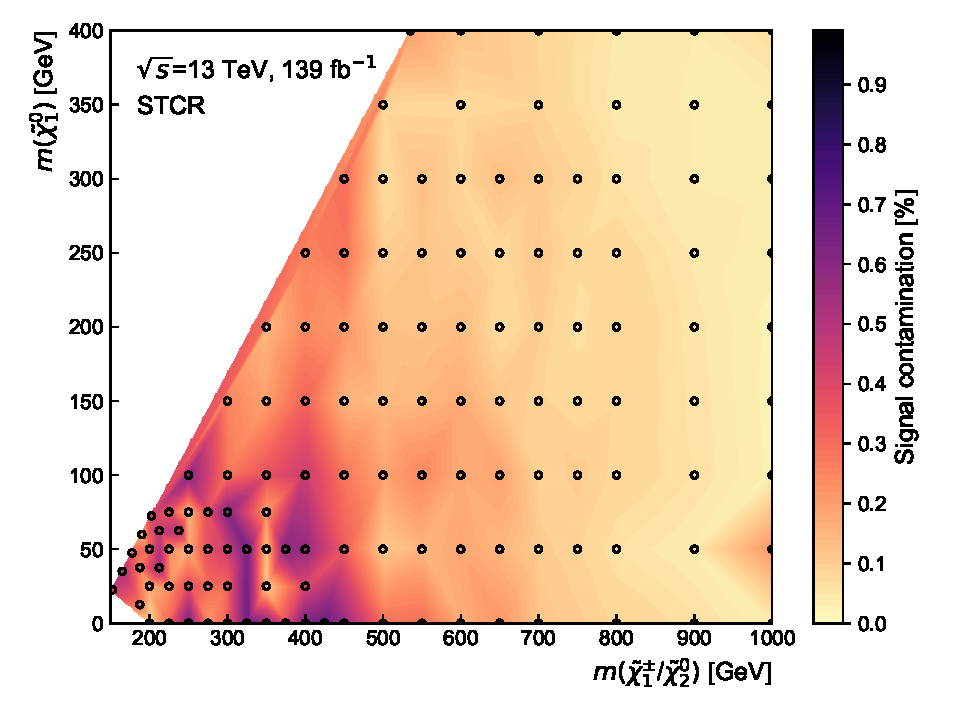
\includegraphics[width=1.0\textwidth]{signal_contamination/plot_STCR}
		\caption{STCR\label{fig:signal_contaminations_STCR}}
	\end{subfigure}\hfill

	\caption{Signal contamination (shown on the \textit{z-axis}) for all \glspl{cr} throughout the signal grid. The space between the signal points (indicated by the black circles) is interpolated using Delaunay triangles.}
	\label{fig:signal_contamination_CR}
\end{figure}


\section{Validation regions}


 \begin{figure}
	\centering
	\begin{subfigure}[b]{0.5\linewidth}
		\centering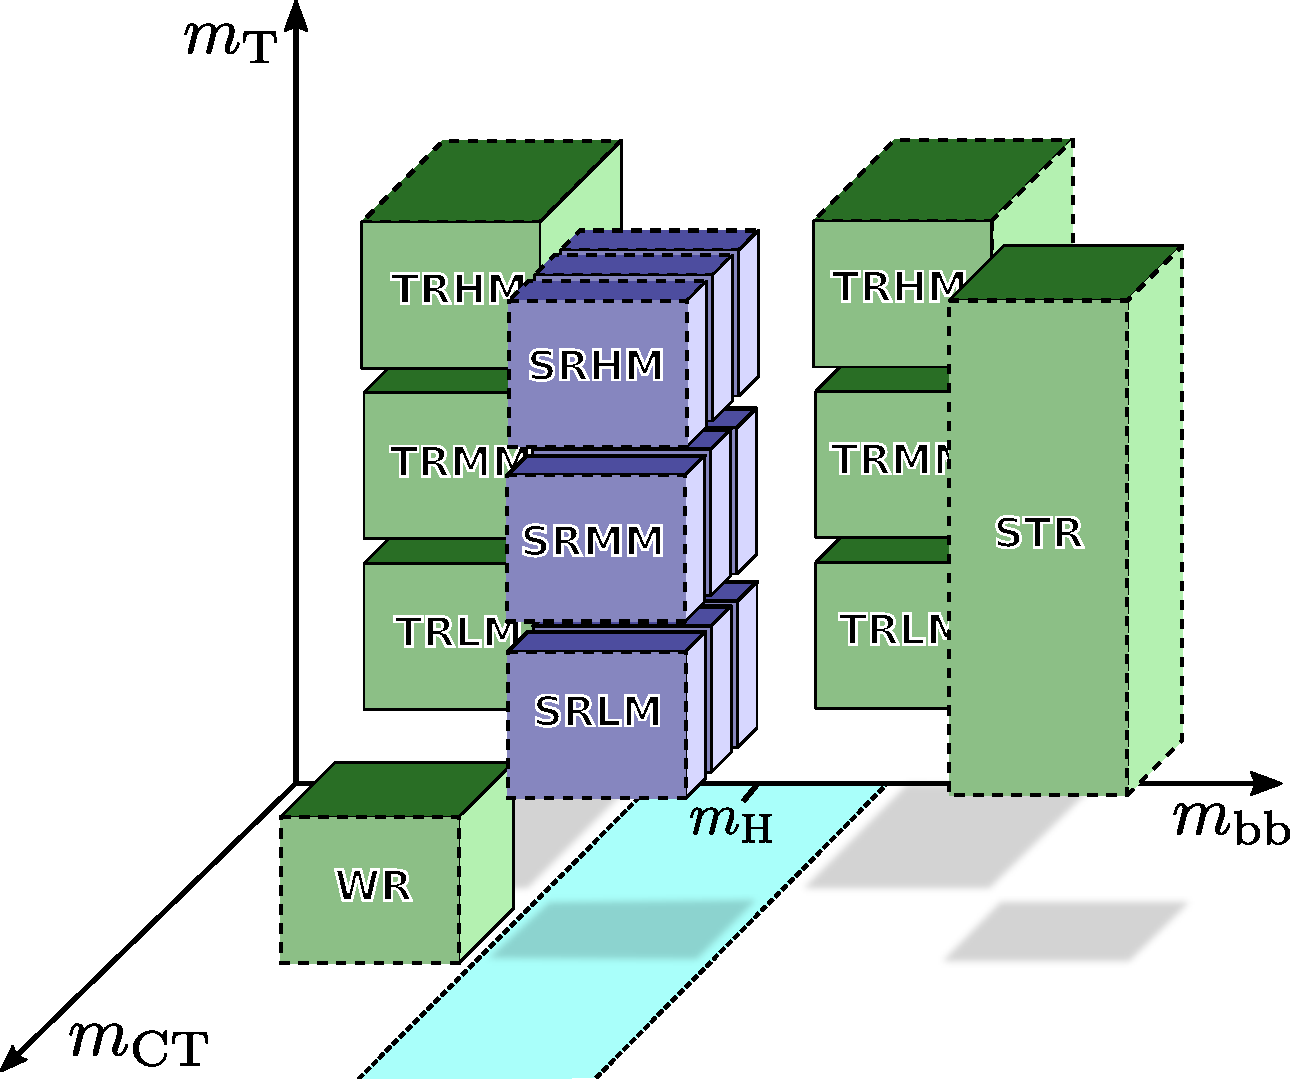
\includegraphics[width=1.0\textwidth]{strategy_5}
		\caption{\label{fig:cr_strategy}}
	\end{subfigure}\hfill
	\begin{subfigure}[b]{0.5\linewidth}
		\centering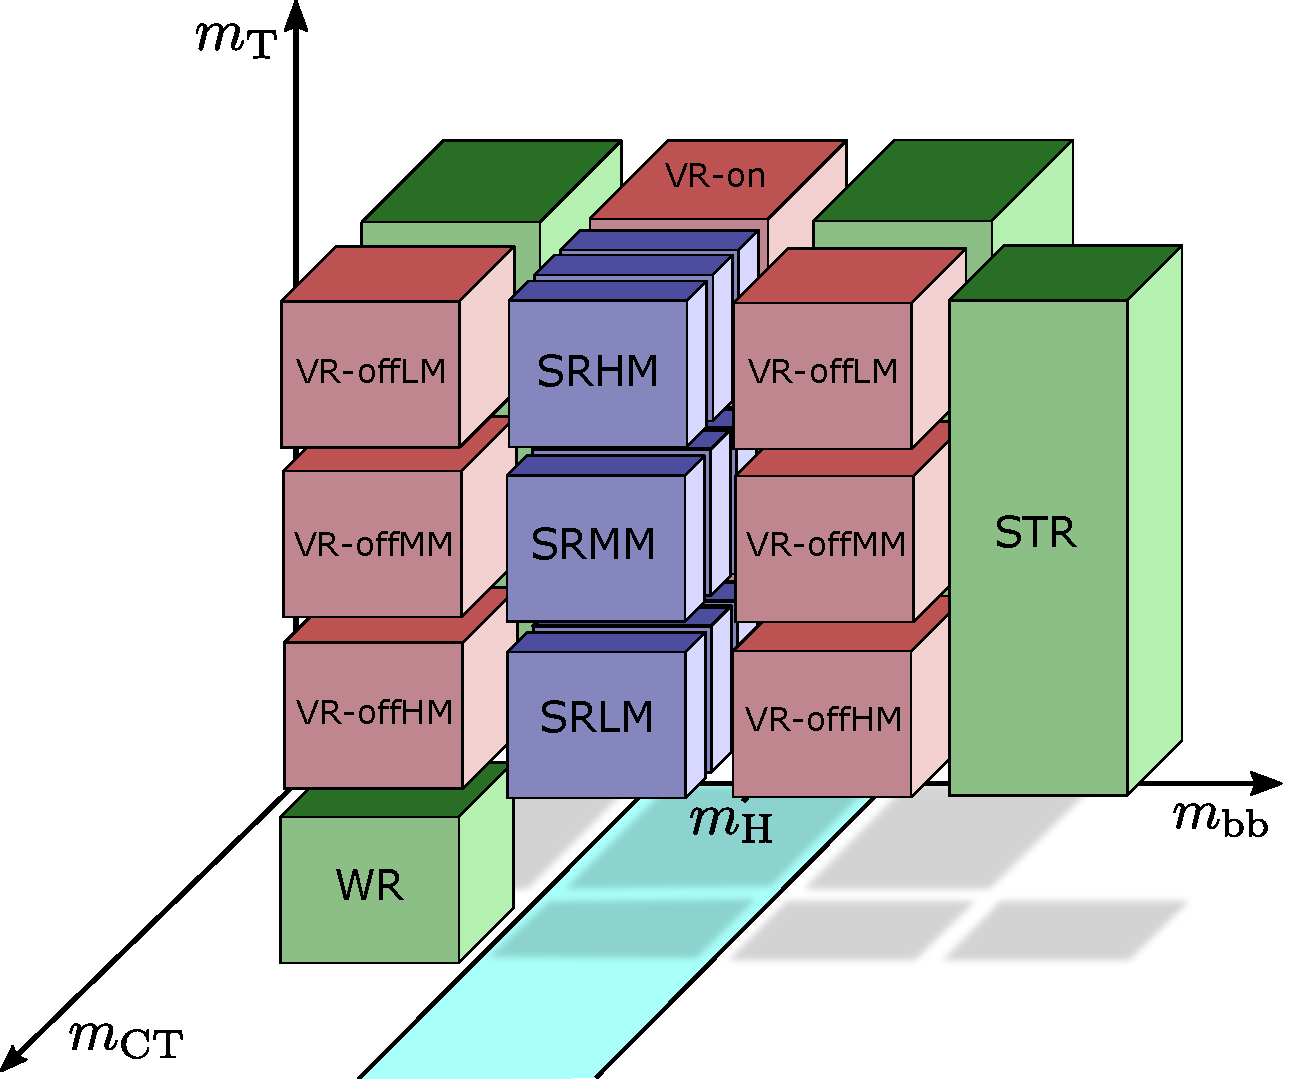
\includegraphics[width=1.0\textwidth]{strategy_7}
		\caption{\label{fig:vr_strategy}}
	\end{subfigure}\hfill

	\caption{Configuration of \subref{fig:cr_strategy} the control regions placed around the signal regions off the $\mbb$ window as well as \subref{fig:vr_strategy} the validation regions in the phase space between the \glspl{cr} and \glspl{sr}. The \glspl{vr} are arranged such that each of the extrapolations can be validated.}
	\label{fig:results_HF_scans}
\end{figure}

Two sets of \glspl{vr} regions are introduced in order to verify the extrapolation over the different distributions. The first set, called VRon is situated on the Higgs boson mass peak but with the $\mct$ requirement inverted to $\mct<\SI{180}{\GeV}$, allowing it to be used for validating the extrapolation in $\mct$. The second set of \glspl{vr} is located on both sides off the Higgs boson mass peak at same values in $\mct$ than the \glspl{sr}. This set of off-peak \glspl{vr}, called VRoff, can be used to validate the extrapolation in $\mbb$. All \glspl{vr} use the same binning in $\mt$ as the \glspl{sr} such that the extrapolation into their respective associated \gls{sr} can be validated. The different bins are consequently called VRonLM, VRonMM VRonHM and VRoffLM, VRoffMM, VRoffHM. The selections defining the \glspl{vr} are summarised in \cref{tab:CRVRdef}.


